\section{Cache}
Der Cache ist ein kleiner aber sehr schneller (Zwischen)Speicher. Er ist viel schneller als der Hauptspeicher. Es können Daten und Tags gespeichert werden.\\
\textcolor{myblue}{Cache Hit}: Gesuchte Adresse im Cache vorhanden\\
\textcolor{myblue}{Cache Miss}: Gesuchte Adresse nicht im Cache\\
\textcolor{myblue}{Berechnung der mittleren Zugriffszeit}: $T_C$ = Zugriffszeit auf Cache, $T_M$ = Zugriffszeit auf Hauptspeicher, $p_C$ = Chance auf Cache Hit\\
% \textcolor{myblue}{Kleinste adressierbare Einheit}: 1 Byte -> zwei Hex-Digits
$E(T)=p_C*T_C+(1-p_C)*T_M$\\
$l$ Länge einer Cachezeile\\
$s$ Grösse des Hauptspeichers\\
$w_n$ Anzahl Wege des Caches auf Stufe n (Anzahl Cacheeinträge)\\
$s_n$ Grösse des Caches auf Stufe n\\\\
$s^{'}_n$ Grösse eines Wegs des Caches auf Stufe n\\
$z_n$ Anzahl Zeilen des Caches auf Stufe n\\\\
$z_n^{'}$ Anzahl Zeilen pro Weg des Caches auf Stufe n\\
$t_n$ Anzahl Bits pro Tag im Cache auf Stufe n\\
$T_n$ Anzahl Bits für alle Tags im Cache auf Stufe n (Overhead)\\
\textcolor{myblue}{Offset}: Bei n-Byte Zeilenlänge --> $2^x = n$ --> x Bit Offset bzw. $l$ in 2er-Potenz und Potenz = Anzahl Byte Offset\\
$s_n = l * z_n$, $z_n = s_n/l$\\
$z_n^{'} = z_n /w_n$,\\
$\text{in FAC } z_n^{'} = z_n$\\
$t_n = l - \text{Bits(2er-Potenz) von } z_n^{'} - \text{ Offset}$,\\
$\text{in FAC }t_n = l - \text{Offset}$\\\\
$T_n = t_n * z_n$\\
\textcolor{myblue}{Speicherstelle des Hauptspeichers auf gleichen Cacheeintrag}: $s/s_n{'} = s/(s_n /w_n ) = s * w_n /s_n$\\
\subsection{Fully Associative Cache(FAC)}
Adressen aufgeteilt in Tags und Offset. Zuerst sucht man die Cachezeile mit dem richtigen Tag, danach sucht man in diesem das richtige Offset. Beste Cache-Leistung, aber teuer da aufwendige HW. Besitzt viele Vergleichsbausteine.
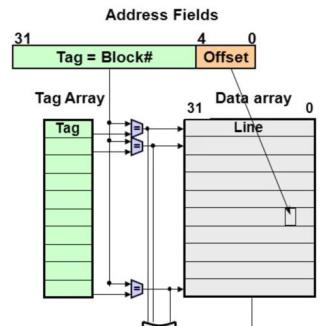
\includegraphics[width=\columnwidth]{fac}
\subsection{Direct Mapped Cache}
Aus dem Main Memory kommen mehrere Einträge in eine Cachezeile. Es ist fixiert in welche Zeile ein Eintrag im Cache hingehört.\\
(blau: Cache Index Bits)\\
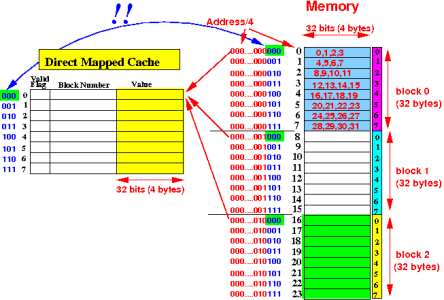
\includegraphics[width=\columnwidth]{dmc}
\textcolor{myblue}{Bsp.} DMC, 16KB Data, 4-word Blöcke, 32 Bit-Adressen.\\
Frage: nach Anz. Bits für den ganzen Cache\\
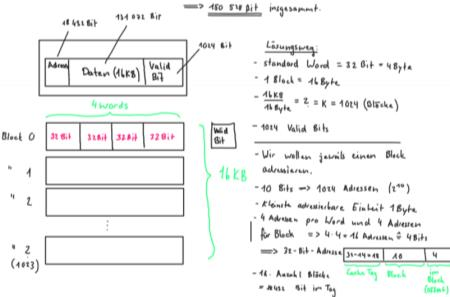
\includegraphics[width=\columnwidth]{dmc_bsp}
\subsection{n-Way Set associative Cache}
Ist ein Kompromiss zwischen Fully Associative Cache und Direct Mapped Cache. Er ist weniger komplex als FAC, hat weniger Kollisionen als DMC ist aber genauso schnell wie DMC. Es gibt für jede Cachezeile n Möglichkeiten(pro Way eine), da n DMCs parallel verwendet werden. Ein Way ist genau eine Cachezeile gross.
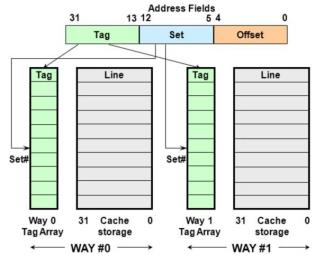
\includegraphics[width=\columnwidth]{sac}
